\documentclass{article}

\usepackage{fancyhdr}
\usepackage{extramarks}
\usepackage{amsmath}
\usepackage{amsthm}
\usepackage{amsfonts}
\usepackage{tikz}
\usepackage{algpseudocode}
\usepackage{listings}
\usepackage{enumitem}
\usepackage{float}
\usepackage[linesnumbered,ruled]{algorithm2e}

\usetikzlibrary{automata,positioning}
\renewcommand{\arraystretch}{1.25}
%
% Basic Document Settings
%

\topmargin=-0.45in
\evensidemargin=0in
\oddsidemargin=0in
\textwidth=6.5in
\textheight=9.0in
\headsep=0.25in

\linespread{1.1}

\pagestyle{fancy}
\lhead{\hmwkAuthorName}
\chead{\hmwkClass\ : \hmwkTitle}
\lfoot{\lastxmark}
\cfoot{\thepage}

\renewcommand\headrulewidth{0.4pt}
\renewcommand\footrulewidth{0.4pt}

\setlength\parindent{0pt}


\newcommand{\hmwkTitle}{Reading Notes}
\newcommand{\hmwkClass}{CS231: Fundamentals of Algorithms}
\newcommand{\hmwkAuthorName}{\textbf{Sophiya Chiang}}

%
% Create Problem Sections
%

\newcommand{\enterProblemHeader}[1]{
    \nobreak\extramarks{}{Reading \arabic{#1} continued on next page\ldots}\nobreak{}
    \nobreak\extramarks{Reading \arabic{#1} (continued)}{Reading \arabic{#1} continued on next page\ldots}\nobreak{}
}

\newcommand{\exitProblemHeader}[1]{
    \nobreak\extramarks{Reading \arabic{#1} (continued)}{Reading \arabic{#1} continued on next page\ldots}\nobreak{}
    \stepcounter{#1}
    \nobreak\extramarks{Reading \arabic{#1}}{}\nobreak{}
}

\setcounter{secnumdepth}{0}
\newcounter{partCounter}
\newcounter{homeworkProblemCounter}
\setcounter{homeworkProblemCounter}{1}
\nobreak\extramarks{Problem \arabic{homeworkProblemCounter}}{}\nobreak{}

%
% Homework Problem Environment
%
% This environment takes an optional argument. When given, it will adjust the
% problem counter. This is useful for when the problems given for your
% assignment aren't sequential. See the last 3 problems of this template for an
% example.
%
\newenvironment{homeworkProblem}[1][-1]{
    \ifnum#1>0
        \setcounter{homeworkProblemCounter}{#1}
    \fi
    \section{Reading \arabic{homeworkProblemCounter}}
    \setcounter{partCounter}{1}
    \enterProblemHeader{homeworkProblemCounter}
}{
    \exitProblemHeader{homeworkProblemCounter}
}

%
% Title Page
%

\title{
    \vspace{2in}
    \textmd{\textbf{\hmwkClass:\ \hmwkTitle}}\\
    \normalsize\vspace{0.1in}\small{Last updated: \today}\\
    \vspace{3in}
}

\author{\hmwkAuthorName}
\date{}

\renewcommand{\part}[1]{\textbf{\large Part \Alph{partCounter}}\stepcounter{partCounter}\\}


\begin{document}

\maketitle

\pagebreak

%Reading for September 11, 2017
\begin{homeworkProblem}
\textbf{Tractability and Asymptotic order of growth}\\
\textbf{Sections 2.1 and 2.2}\\\\
\underline{\textbf{2.1 Computational Tractability}}
\begin{itemize}
\item
\textit{Worst-case} running time: A bound on the largest possible running time the algorithm could have over all inputs of a given size $N$
\item An algorithm is efficient if it achieves qualitatively better worst-case performances, at an analytical level, than brute-force search.
\item An algorithm is efficient if it has a polynomial running time: lower-degree polynomials exhibit better scaling behavior than higher-degree polynomials.
\end{itemize}

\underline{\textbf{2.2 Asymptotic Order of Growth}}
\begin{itemize}
\item An algorithm's worst-case running time on inputs of size $n$ grows at a rate that is at most proportional to some function $f(n)$. The function $f(n)$ becomes a bound on the running time of the algorithm.
\item
\textit{Asymptotic upper bounds:} $T(n)$ is $O(n)$ ($T(n)$ is order of $n$) if, for sufficiently large $n$ the function $T(n)$ is bounded above by a constant multiple of $f(n)$. So, $T(n)$ is \textit{asymptotically upper-bounded by $f(n)$}.
\begin{center}
    $T(n) \in O(n)$ if $\exists (c > 0$ and $n_0 \geq 0)$ $\mid$ \ $\forall n \geq n_0, T(n) \leq c \cdot f(n)$
\end{center}

\item
\textit{Asymptotic lower bounds:} $T(n)$ is $\Omega(n)$ if, for arbitrarily large input size $n$, the function $T(n)$ is at least a constant multiple of $f(n)$. So, $T(n)$ is \textit{asymptotically lower-bounded by $f(n)$}.
\begin{center}
    $T(n) \in O(n)$ if $\exists (\epsilon > 0$ and $n_0 \geq 0)$ $\mid$ \ $\forall n \geq n_0, T(n) \geq \epsilon \cdot f(n)$
\end{center}

\item
\textit{Asymptotically tight bounds:} If a function is both $O(n)$ and $\Omega(n)$, then $T(n)$ is $\Theta(n)$. They characterize the worse-case performance of an algorithm precisely up to constant factors. So, $f(n)$ is an \textit{asymptotically tight bound for $T(n)$}. One can sometimes obtain an asymptotically tight bound directly by computing the limit as $n$ goes to infinity. If the ratio of functions $f(n)$ and $g(n)$ converges to a positive constant as $n$ goes to infinity, then $f(n) \in \Theta(g(n))$
\begin{center}
    $T(n) \in O(n)$ if $\exists (\epsilon > 0$ and $n_0 \geq 0)$ $\mid$ \ $\forall n \geq n_0, T(n) \geq \epsilon \cdot f(n)$
\end{center}

\item 
\textbf{Properties of Asymptotic Growth Rates:}
\textit{Transitivity:} If a function $f$ is asymptotically upper-bounded by a function $g$, and $g$ is asymptotically upper-bounded by $h$, then $f$ is asymptotically upper-bounded by $h$. 
\begin{enumerate}
\item
If $f = O(g)$ and $g = O(h)$, then $f = O(h)$.
\item
If $f = \Omega(g)$ and $g = \Omega(h)$, then $f = \Omega(h)$.
\item 
If $f = \Theta(g)$ and $g = \Theta(h)$, then $f = \Theta(h)$.
\item
Suppose that $f$ and $g$ are two functions such that for some other function $h$, we have $f=O(h)$ and $g=O(h)$. Then, $f + g = O(h)$.
\item 
Let $k$ be  fixed constant, and let $f_1, f_2,\ldots, f_k$ and $h$ be functions such that $f_i = O(h) \forall i$. Then, $f_1 + f_2+\ldots+ f_k = O(h)$.
\item
Suppose that $f$ and $g$ are two functions (taking non-negative values) such that for $g = O(f)$. Then, $f + g = \Theta(f)$. $f$ is an asymptotically tight bound for the combined function $f + g$.

\end{enumerate}
\end{itemize}
\end{homeworkProblem}
\pagebreak

%Reading for September 14, 2017
\begin{homeworkProblem}
\textbf{The Stable Matching Problem}\\
\textbf{Sections 2.3}\\\\
\underline{\textbf{2.3 Implementing the Stable Matching Algorithm Using Lists and Arrays}}
\begin{itemize}
\item
Consider how the data will be represented and manipulated in an implementation of the algorithm, so as to bound the number of computational steps it takes.
\item
Considering the Gale-Shapely Matching algorithm, the algorithm terminates in at most $n^2$ iterations and to get an implementation with worst-case running time of $O(n^2)$, we need to be able to implement each iteration in constant time by counting actual computational steps rather than simply the total number of iterations using arrays and lists.
\item
We need to be able to do each of these four steps of the algorithm in constant time:
\begin{enumerate}
    \item Identify a free man. \textbf{Implemented in $O(1)$ time}
        \begin{itemize}
            \item Maintaining the set of free men as a linked list.
            \item When selecting a free man, we take the first man $m$ on this list. 
            \item We delete $m$ from the list if he becomes engaged, and possibly insert a different man $m'$, if some other man $m'$ becomes free. $m'$ can be inserted at the front of the list at constant time in this case.
        \end{itemize}
    \item For a man $m$, we need to identify the highest-ranked woman to whom he has not yet proposed. \textbf{Implemented in $O(1)$ time}
        \begin{itemize}
        \item 
        Maintain an extra array $Next$ that indicates for each man $m$ the position of the next woman he will propose to on his list.
        \item We initialize $Next[m] = 1$ for all men $m$. If a man $m$ needs to propose to a woman, he'll propose to $w = ManPref[m, Next[m]]$
        \item Once he proposes to $w$, we increment the value of $Next[m]$ by one, regardless of whether $w$ accepts the proposal.
        \end{itemize}
    \item For a woman $w$, we need to decide if $w$ is currently engaged, and if she is, we need to identify her current partner. \textbf{Implemented in $O(1)$ time}
        \begin{itemize}
            \item Assuming man $m$ proposes to woman $w$, we need to identify the man $m'$ that $w$ is currently engaged to (if exists).
            \item Maintain an array $Current$ of length $n$, where $Current[w]$ is the woman $w$'s current partner $m'$.
            \item We set $Current[w]$ to a special null value when woman $w$ is not currently engaged.
            \item Initialize $Current[w]$ to null value at the start of the algorithm.
        \end{itemize}
    
    \item For a woman $w$, and two men $m$ and $m'$, we need to be able to decide in constant time, which of $m$ or $m'$ is preferred by $w$. \textbf{Implemented in $O(n^2)$ time}
        \begin{itemize}
            \item At the start of algorithm, we create an $n\times n$ array $Ranking$, where $Ranking[w,m]$ contains the rank of man $m$ in the sorted order of $w$'s preferences. 
            \item By a single pass through $w$'s preference list, we can create this array in linear time for each woman, for a total initial time investment proportional to $n^2$.
            \item To decide which of $m$ or $m'$ is preferred by $w$, we simply compare values $Ranking[w,m]$ to $Ranking[w,m']$.
        \end{itemize}
\end{enumerate}
\end{itemize}
\end{homeworkProblem}
\pagebreak

%Reading for September 18, 2017
\begin{homeworkProblem}
\textbf{Priority Queues}\\
\textbf{Sections 2.5}\\\\
\underline{\textbf{2.5 Priority Queues}}
\begin{itemize}
    \item For the Stable Matching algorithm, we need to maintain a dynamically changing set $S$ (set of free men in this case).
    \item We want to be able to add and delete elements from the set $S$, and we want to be able to select an element $S$ when the algorithm calls for it.
    \item A priority queue is designed for applications in which elements have a \textit{priority value (key)} and each time we need to select an element from $S$, we want to take the one with hightest priority.
    \item Maintains a set of elements $S$, where element $v \in S$ has an associated value $key(v)$ that denotes the priority of element $v$, where smaller keys represent higher priorities.
    \item Supports the addition and deletion of elements from the set, and also the selection of the element with smallest key. 
    \item Each process has a priority/urgency, but processes do not arrive in order of their priorities.
    \item Implementation of a priority queue containing at most $n$ elements at any time so that elements can be added and deleted, and the element with minimum key selected, in $O(log (n))$ time per operation.
    \item \textit{A sequence of $O(n)$ priority queue operations can be used to sort a set of $n$ numbers}\\
    \textbf{Proof: }Set up a priority queue $H$, and insert each number into $H$ with its value as a key. Then extract the smallest number one by one until all numbers have been extracted. This way, the numbers will come out of the priority queue in sorted order.
    \item So with a priority queue that can perform insertion and deletion of minima $O(log(n))$ time per operation, we can sort $n$ numbers in $O(n(log(n)))$ time.
    
    \item\textbf{Heap} - Implementing a Priority Queue
    \begin{itemize}
        \item The heap data structure combines the benefits of a sorted array and list for purposes of this application.
        \item Conceptually, we can think of it as a balanced binary tree. Where the tree will have a root, and each node can have up to two children (A left and a right child).
        \item \textit{Heap order: }If the key of any element is at least as large as the key of the element at its parent node in the tree.
        \begin{center}
        For every element $v$, at a node $i$, the element $w$ at $i$'s parent satisfies $key(w) \leq key(i)$.
        \end{center}
        \item If a bound $N$ is known in advance on the total number of elements that will ever be in the heap at any one time, we can maintain the heap in an array $H$ indexed by $i=1, 2, \ldots, N$.
        \item We can think of heap nodes as corresponding to the positions of the array, with $H[1]$ being the root.
        \item For any node at position $i$, the children are the nodes at position $leftChild(i) = 2i$ and $rightChild(i) = 2i+1$. And the parent of a node at position $i$ is at position $parent(i) = i/2$.
        \item If the heap has $n<N$ elements at some time, we can use the first $n$ positions of the array to store the $n$ heap elements. Using $length(H)$ to denote the number of elements in $H$. So the heap is balanced at all times.
    \end{itemize}
    \item\textbf{Implementing the Heap Operations:}
    \begin{itemize}
        \item The heap element with smallest key is at the root, so it takes $O(1)$ time to identify the minimal element. 
        \item Adding element $v$ to final position $i = n + 1$ and fixing the heap with \textbf{Heapify-up} by moving element $v$ towards the root. 
        \item The \textbf{Heapify-up} procedure fixes the heap property in $O(log(n))$ time, assuming that the array $H$ is almost a heap with the key $H[i]$ too small. Using the following procedure, we can insert a new element in a heap of $n$ elements in $O(log(n))$ time.
        \begin{lstlisting}
        Heapify-up(H,i):
            If i > 1 then
                let j = parent(i) = (1/2)
                If key[H[i]] < key[H[j]] then
                    swap the array entries H[i] and H[j]
                    Heapify-up(H,j)
                Endif
            Endif
        \end{lstlisting}
        Proof by induction on pp.62 of textbook.
        \item Procedure \textbf{Heapify-down} swaps the element at position $i$ with one of its children and proceeds down the tree recursively.
        \item \textbf{Heapify-down(H,i)} fixes the heap property in $O(log(n))$ time, assuming that $H$ is almost a heap with the key value of $H[i]$ too big. Using \textbf{Heapify-up} or \textbf{Heapify-down}, we can delete a new element in a heap of n elements in $O(log(n))$ time.
        \begin{lstlisting}
        Heapify-down(H,i):
            Let n = length(H)
            If 2i > n then
                Terminate with H unchanged
            Else if 2i < n then
                Let left = 2i, and right = 2i + 1
                Let j be the index that minimizes key[H[left]] and key[H[right]]
            Else if 2i = n then
                Let j = 2i
            Endif
            If key[H[j]] < key[H[i]] then
                Swap the array entries H[i] and H[j]
                Heapify-down[H, j]
            Endif
        \end{lstlisting}
        Proof by reverse induction on value i on pp.64 of textbook.
    \end{itemize}
    \item\textbf{Implementing Priority Queues with Heaps}\\
    If the priority queue is constrained to hold at most $N$ elements at any point in time.
    \begin{itemize}
        \item $StartHeap(N)$ returns an empty heap $H$ that is set up to store at most $N$ elements. This operation takes $O(n)$ time, as it involves initializing the array that will hold the heap.
        \item $Insert(H,v)$ inserts the item $v$ into the heap $H$. If the heap currently has elements, this takes $O(log(n))$ time.
        \item $FindMin(H)$ identifies the minimum element in the heap $H$ but does not remove it. This takes $O(1)$ time.
        \item $Delete(H,i)$ deletes the element in heap position $i$. This is implements in $O(log(n)$ time for heaps that have $n$ elements.
        \item $ExtractMin(H)$ identifies and deletes and element with minimum key value from a heap. This is a combination of the previous two operations, so this takes $O(log(n))$ time.
    \end{itemize}
    To be able to access given elements of the priority queue efficiently, we simply maintain an additional array $Position$ that stores the current position of each element (each node) in the heap.
    \begin{itemize}
        \item To delete the element $v$, we apply $Delete(H, Position[v])$. Maintaining this array does not increase the overall running time, so we can delete an element $v$ from a heap with $n$ notes in $O(log(n))$ time.
        \item $ChangeKey(H,v,\alpha)$ which changes the key value of element $v$ to $key(v) = \alpha$. We can implement this operation in $O(log(n))$ time by first identifying the position of element $v$ in the array by using the $Position$ array. Once we have defined the position of element $v$, we change the key and then apply \textbf{Heapify-up} or \textbf{Heapify-down} as appropriate.
    \end{itemize}
\end{itemize}
\end{homeworkProblem}
\pagebreak

\begin{homeworkProblem}
\textbf{Graphs}\\
\textbf{Sections 3.1 and 3.2}\\\\
\underline{\textbf{3.1 Basic Definitions}}
\begin{itemize}

    \item A graph G encodes a pairwise relationship among objects: a collection $V$ of \textit{nodes} and a collection $E$ of \textit{edges}.
    \item An edge $e \in E$ is a 2-element subset of $V: e = \{u,v\}$ for some $u, v \in V$ where $u, v$ are the \textit{ends} of $e$.
    \item Undirected graphs: indicate a symmetric relationship between the ends of the edges in a graph.
    \item Directed graphs: consists of a set of nodes $V$ and a set of \textit{directed edges} $E'$, where each $e' \in E'$ is an ordered pair $(u,v)$.
    \item A path in an undirected graph $G=(V,E)$ is a sequence $P$ of nodes $v_1, v_2, v_3, \ldots, v_{k-1}, v_k$ such that each consecutive pair $v_i, v_{i+1}$ is joined by an edge in $G$.
        \begin{itemize}
            \item Simple path: if all vertices are distinct from one another
            \item Cycle: is a path $v_1, v_2, v_3, \ldots, v_{k-1}, v_k$ where $k>2$, the first $k-1$ nodes are distinct, and $v_1 = v_k$.
        \end{itemize}
    \item Connected graph: if for every pair of nodes $u, v$ there is a path from $u$ to $v$.
    \item Distance between two nodes $u, v$: the minimum number of edges in a $u-v$ path.
    \item Tree: An undirected graph that is connected and does not contain a cycle.
    \item Every $n-node$ tree has exactly $n-1$ edges.
    \item Let $G$ be an undirected graph on $n$ nodes. Any of two of the following statements implies the third.
    \begin{itemize}
        \item G is connected.
        \item G does not contain a cycle.
        \item G has $n-1$ edges.
    \end{itemize}
\end{itemize}

\underline{\textbf{3.2 Graph Connectivity and Graph Traversal}}
\begin{itemize}
    \item $s-t$ connectivity problem/Maze solving problem: finding a path, if any, from $s$ to $t$ in $G$.
    \item Breadth-first search (BFS)
    \begin{itemize}
        \item Explore outward from $s$ in all possible directions, including nodes that are joined by an edge to $s$. Continue until no new nodes are encountered.
        \item Layers $L_1, L_2, L_3,\ldots$: 
        \begin{itemize}
            \item Layer $L_0$ is the set consisting just of $s$
            \item Layer $L_1$ consists of al nodes that are neighbors of $s$.
            \item Assuming we have defined layers $L_1, \ldots, L_j$, then layer $L_{j+1}$ consists of all nodes that do not belong to an earlier later and that have an edge to a node in layer $L_j$.
            \item A node fails to appear in any of the layers iff there is no path to it.
        \end{itemize}
        \item BFS determines the nodes that $s$ can reach and computes the shortest paths to them.
        \item For each $j \geq 1$, Layer $L_j$ produced by BFS consists of all nodes at distance exactly $j$ from $s$. There is a path from $s$ to $t$ iff $t$ appears in some layer.
        \item \textit{Breadth-first search tree}: BFS produces a tree $T$ rooted at $s$ on the set of nodes reachable from $s$: Let $T$ be a breadth-first search tree, let $x$ and $y$ be nodes in $T$ belonging to layers $L_i$ and $L_j$ respectively, and let $(x, y)$ be an edge of $G$. Then $i$ and $j$ differ at most by 1.
    \end{itemize}
    \item Depth-first search (DFS)
    \begin{itemize}
        \item We can invoke DFS from any starting point but maintain global knowledge of which nodes have already been explored.
        \item Let $T$ be a depth-first search tree, let $x$ and $y$ be nodes in $T$, and let $(x, y)$ be an edge of $G$ that is not an edge of $T$. Then one of $x$ or $y$ is an ancestor of the other.
    \end{itemize}
    \item For any two nodes $s$ and $t$ in a graph, their connected components are either identical or disjoint.
\end{itemize}

\end{homeworkProblem}
\pagebreak

\begin{homeworkProblem}
\textbf{Graph traversal}\\
\textbf{Sections 3.3 and 3.4}\\\\
\underline{\textbf{3.3 Implementing Graph Traversal Using Queues and Stacks}}
\begin{itemize}
    \item Basic representation of graphs: By an \textit{adjacency matrix} and by an \textit{adjacency list}.
    \item A graph $G=(V,E)$, let $|V| = n$ and $|E| = m$. With at most one edge between any pair of nodes, $m \leq \binom{n}{2} \leq n^2$.
    \item A connected graph must have at least $m \geq n-1$ edges.
    \item Linear time for graph search: $O(m+n)$ time to read the input.
    \item For connected graphs: $O(m+n) \equiv O(m)$ since $m\geq n-1$.
    \item\textbf{Adjacency matrix:} Consider a graph $G = (V , E)$ with $n$ nodes, and assume the set of nodes is $V = \{1,\ldots, n\}$. 
    \begin{itemize}
        \item The adjacency matrix is an $n\times n$ matrix $A$ where $A[u,v]$. is equal to 1 if the graph contains the edge $(u,v)$ and 0 otherwise.
        \item If the graph is undirected, the matrix $A$ is symmetric, with $A[u,v] = A[v,u]$ for all nodes $u, v \in V$.
        \item Can check in $O(1)$ time if a given edge $(u,v)$ is present in the graph.
        \item Representation takes $\Theta(n^2)$ space. When the graph has many fewer edges than $n^2$, more compact representations are possible.
        \item Many graph algorithms need to examine all edges incident to a given node $v$ and in the matrix, you have to consider all other nodes $w$, and checking the matrix entry $A[v, w]$ to see whether the edge $(v, w)$ is present in $\Theta(n)$ time. Worst case, $v$ may have $\Theta(n)$ incident edges, so checking all edges will take $\Theta(n)$ time regardless of the representation. 
    \end{itemize}
    \item\textbf{Adjacency list:} Array $adj$ where $Adj[v]$ is a record containing a list of all nodes adjacent to node $v$. 
    \begin{itemize}
        \item Works better for sparse graphs with fewer than $n^2$ edges.
        \item For an undirected graph $G = (V, E)$, each edge $e = (v, w) \in E$ occurs on two adjacency lists: node w appears on the list for node $v$, and node $v$ appears on the list for node $w$.
        \item Requires only $O(m+n)$ space: array of pointers of length $n$ to set up the lists in $Adj$, and then we need space for all the lists - each edge $e = (v,w)$ appears in exactly two of the lists: one for $v$ and one for $w$. So the total length of all lists is $2m = O(m)$.
        \item Degree $n_v$ of a node $v$ is the number of incident edges it has.
        \item Length of the list at $Adj[v]$ is $n_v$, so the total length over all nodes is $O(\sum_{v\in V} n_v)$.
        \item Sum of the degrees in a graph: $O(\sum_{v\in V} n_v) = 2m$.
        \item To check if a particular edge $(u,v)$ is present in the graph: in $O(n_v)$ - by following the pointers on $u$'s adjacency list to see if edge $v$ occurs on the list.
    \end{itemize}

    \item\textit{Discovering} a node $v$ - the first time it is seen, when the algorithm finds an edge leading to $v$.
    \item\textit{Exploring} a node $v$ - when all the incident edges to $v$ are scanned, resulting in the potential discovery of further nodes.
    \item Implement queues and stacks using doubly-linked list - always selecting the first element on our list, different in where we insert a new element.
    \item\textbf{Queue: }A set from which we extract elements in first-in, first-out order (FIFO) - select elements in the same order in which they were added. Elements are added to the end of the list as the last element. \textit{Implement BFS to select which node to consider next.}
    \begin{itemize}
        \item Implementing BFS:
        \begin{lstlisting}
BFS(s):
    Set Discovered[s] = true and Discovered[v] = false for all other v 
    Initialize L[0] to consist of the single element s
    Set the layer counter i = 0
    Set the current BFS tree T = empty set
    While L[i] is not empty
        Initialize an empty list L[i + 1] 
        For each node u ∈ L[i]
            Consider each edge (u, v) incident to u 
            If Discovered[v] = false then
                Set Discovered[v] = true
                Add edge (u, v) to the tree T
                Add v to the list L[i+1] 
            Endif
        Endfor
        Increment the layer counter i by one 
    Endwhile
        \end{lstlisting}
        \item The above implementation of the BFS algorithm runs in time $O(m + n)$ (i.e., linear in the input size), if the graph is given by the adjacency list representation.
    \end{itemize}
    
    \item\textbf{Stack: }A set from which we extract elements in last-in, first-out order (LIFO) - we select an element that was added most recently. A new element is placed in the first position on the list. \textit{Implement DFS.}
    \begin{itemize}
        \item Implementing DFS:
        \begin{lstlisting}
DFS(s):
    Initialize S to be a stack with one element s
    While S is not empty
        Take a node u from S
        If Explored[u] = false then
            Set Explored[u] = true
            For each edge (u,v) incident to u
                Add v to the stack S
            Endfor
        Endif
    Endwhile
        \end{lstlisting}
        \item The above algorithm implements DFS, in the sense that it visits the nodes in exactly the same order as the recursive DFS procedure in the previous section (except that each adjacency list is processed in reverse order).
        \item The above implementation of the DFS algorithm runs in time $O(m + n)$ (i.e., linear in the input size), if the graph is given by the adjacency list representation.
    \end{itemize}
\end{itemize}
\pagebreak

\underline{\textbf{3.4 Testing Bipartite-ness}}
\begin{itemize}
\item\textbf{Bipartite graph:} it is one where the node set $V$ can be partitioned into sets $X$ and $Y$ in such a way that every edge has one end in $X$ and the other end in $Y$
\item If a graph $G$ is bipartite, then it cannot contain an odd cycle.
\item To determine whether $G$ is bipartite, we can also show that we can find an odd cycle in $G$ whenever it is not bipartite.
\item We perform BFS, colors $s$ red, all of later $L_1$ blue, all of layer $L_2$ red, and so on - coloring odd-numbered layers blue and even-numbered layers red. We implement this by adding an extra array $Color$ over the nodes. Whenever we get to a step in BFS where we are adding a node $v$ to a list $L[i+1]$, we assign $Color[v] = red$ if $i+1$ is an even number and $Color[v] = blue$ if $L[i+1]$ is an odd number. At the end of the procedure we scan all the edges and determine whether there is any edge for which both ends received the same color. Thus the coloring algorithm is $O(m+n)$, as it is for BFS.

\item Let $G$ be a connected graph, and let $L_1, L_2,\ldots$ be the layers produced by BFS starting at node $s$. Then exactly one of the following two things must hold:
    \begin{itemize}
        \item There is no edge of $G$ joining two nodes of the same layer. In this case $G$ is a bipartite graph in which the nodes in even-numbered layers can be colored red, and the nodes in odd-numbered layers can be colored blue.
        \item There is an edge of $G$ joining two nodes of the same layer. In this case, $G$ contains an odd-length cycle, and so it cannot be bipartite.
    \end{itemize}
\end{itemize}
\end{homeworkProblem}
\pagebreak

\begin{homeworkProblem}
\textbf{Data Structures Review}

\underline{\textbf{Data Structures Overview}}
\begin{enumerate}
    \item Array
    \begin{itemize}
        \item Store homogeneous elements at contiguous locations
        \item Size of an array must be provided before storing data. Let size be $n$.
        \item Accessing Time: $O(1)$ [because elements are stored at contiguous locations]
        \item Search Time: $O(n)$ for Sequential Search; $O(Log(n))$ for Binary Search [If sorted]
        \item Insertion Time: $O(n)$ [Worst case if inserted at the beginning of array - shifting all of the elements]
        \item Deletion Time: $O(n)$ [Worst case deleting at the beginning of the array - shifting all of the elements]
    \end{itemize}
    
    \item Linked List
    \begin{itemize}
        \item Each element is a separate object. Each element contains the data and a reference to the next node.
        \item\textbf{Singly Linked List: }Every node stores reference of next node in list. Last node has reference NULL.
        \item\textbf{Doubly Linked List: }Two references associated with each node. One reference points to the next node and one points to the previous node. can traverse in both direction. NULL at the end.
        \item\textbf{Circular Linked List: }All nodes are connected to form a circle. No NULL at the end. Can be singly or doubly linked. Any node can be the starting node.
        \item Accessing time of an element : $O(n)$
        \item Search time of an element : $O(n)$
        \item Insertion of an Element : $O(1)$ [If we are at the position where we have to insert an element] 
        \item Deletion of an Element : $O(1)$ [If we know address of node previous to the node to be deleted] 
    \end{itemize}
    
    \item Stack
    \begin{itemize}
        \item Last in, first out (LIFO) 
        \item Abstract data type as a collection of elements
        \item Operations: push (adds an element to collection), pop (removes the last element that was added) - both occur at the top of the stack.
        \item Can be implemented as array or linked list
        \item Insertion : $O(1)$
        \item Deletion :  $O(1)$
        \item Access Time : $O(n)$ [Worst Case] Insertion and Deletion are allowed on one end. 
    \end{itemize}
    
    \item Queue
    \begin{itemize}
        \item First in, first out (FIFO)
        \item Abstract data type as a collection of elements
        \item Operations: enqueue (adds an element to the end of collection), dequeue (removes the first element that was added).
        \item Can be implemented as array or linked list    
        \item Insertion : $O(1)$
        \item Deletion :  $O(1)$
        \item Access Time : $O(n)$ [Worst Case] Insertion and Deletion are allowed on one end. 
    \end{itemize}

    \item Binary Tree
    \begin{itemize}
        \item Hierarchical data structure
        \item Each node has at most two children: left child and right child
        \item Usually implemented with Linked Lists, but possible with arrays too
        \item Represented by a pointer to root. If tree is empty, root = NULL.
        \item A node contains: Data, pointer to left child, and pointer to right child
        \item Traversal: 
        \begin{enumerate}
            \item Depth First Traversal: Inorder (Left-Root-Right), Preorder (Root-Left-Right) and Postorder (Left-Right-Root)
            \item Breadth First Traversal: Level Order Traversal
        \end{enumerate}
        \item The maximum number of nodes at level $l = 2^{l-1}$.
        \item Maximum number of nodes = $2^{h}-1$, where $h$ is the height of the tree (Max. number of nodes on root to leaf path)
        \item Minimum possible height =  $ceil(Lg(n+1))$ (number of leaf nodes is always one more than nodes with two children)
        \item Time Complexity of Tree Traversal: O(n) - consider degenerate trees
    \end{itemize}
    
    \item Binary Search Tree    
    \begin{itemize}
        \item A Binary tree with three additional properties:
        \begin{itemize}
            \item Left subtree of a node contains only nodes with keys less than the node's key
            \item The right subtree of a node contains only nodes with keys greater than the node's key.
            \item The left and right subtree each must also be a binary search tree.
        \end{itemize}
        \item Search : $O(h)$
        \item Insertion : $O(h)$
        \item Deletion : $O(h)$
        \item Extra Space : $O(n)$ for pointers
        \item $h$: Height of BST and $n$: Number of nodes in BST
        \item If Binary Search Tree is height balanced, then $h = O(Log(n))$ \item Self-Balancing BSTs such as AVL Tree, Red-Black Tree and Splay Tree make sure that height of BST remains $O(Log(n))$
        \item BST provide moderate access/search (quicker than Linked List and slower than arrays).
        \item BST provide moderate insertion/deletion (quicker than Arrays and slower than Linked Lists).
    \end{itemize}
    
    \item Binary Heap
    \begin{itemize}
        \item A Binary tree with two additional properties:
        \begin{itemize}
            \item It's a complete tree (All levels are completely filled except possibly the last level and the last level has all keys as left as possible). This property of Binary Heap makes them suitable to be stored in an array.
            \item A Binary Heap is either Min Heap or Max Heap. In a Min Binary Heap, the key at root must be minimum among all keys present in Binary Heap. The same property must be recursively true for all nodes in Binary Tree. Max Binary Heap is similar to Min Heap. It is mainly implemented using array.
        \end{itemize}
        \item Get Minimum in Min Heap: $O(1)$ [Or Get Max in Max Heap]
        \item Extract Minimum Min Heap: $O(Log(n))$ [Or Extract Max in Max Heap]
        \item Decrease Key in Min Heap: $O(Log(n))$  [Or Increase key in Max Heap]
        \item Insert: $O(Log(n))$
        \item Delete: $O(Log(n))$
    \end{itemize}
    
    \item Hashing
    \begin{itemize}
        \item\textbf{Hash function: }A function that converts a given big input key to a small practical integer value. The mapped integer value is used as an index in hash table.
        \item Usually efficiently computable and uniformly distributes the keys (each table position equally likely for each key)
        \item\textbf{Hash table: }An array that stores pointers to records corresponding to a given phone number. An entry in hash table is NIL if no existing phone number has hash function value equal to the index for the entry.
        \item\textbf{Collision Handling: }Since a hash function gets us a small number for a key which is a big integer or string, there is possibility that two keys result in same value. The situation where a newly inserted key maps to an already occupied slot in hash table is called collision and must be handled using some collision handling technique.
        \item\textbf{Chaining:} The idea is to make each cell of hash table point to a linked list of records that have same hash function value. Chaining is simple, but requires additional memory outside the table.
        \item\textbf{Open Addressing:} In open addressing, all elements are stored in the hash table itself. Each table entry contains either a record or NIL. When searching for an element, we one by one examine table slots until the desired element is found or it is clear that the element is not in the table.
        \item Space: $O(n)$
        \item Search: $O(1)$ [Average]; $O(n)$ [Worst case]
        \item Insertion: $O(1)$ [Average]; $O(n)$ [Worst Case]
        \item Deletion: $O(1)$ [Average]; $O(n)$ [Worst Case]
        \item Hashing seems better than BST for all the operations. But in hashing, elements are unordered and in BST elements are stored in an ordered manner. Also BST is easy to implement but hash functions can sometimes be very complex to generate. In BST, we can also efficiently find floor and ceiling of values.
    \end{itemize}
    
    \item Graph
    \begin{itemize}
        \item Time Complexities in case of Adjacency Matrix:
        \begin{itemize}
            \item Traversal: (By BFS or DFS) $O(V^2)$
            \item Space: $O(V^2)$
        \end{itemize}
        \item Time Complexities in case of Adjacency List :
        \begin{itemize}
            \item Traversal: $O(|E|log(|V|))$ (By BFS or DFS) 
            \item Space: $O(|V|+|E|)$
        \end{itemize}
    \end{itemize}
    
\end{enumerate}
\end{homeworkProblem}
\pagebreak

\begin{homeworkProblem}
\textbf{Connectivity in Graphs and Topological Ordering}\\
\textbf{Sections 3.5 and 3.6}\\\\
\underline{\textbf{3.5 Connectivity in Directed Graphs}}
\begin{itemize}
    \item In a directed graph, the edge $(u,v)$ has a direction from $u$ to $v$, so the relationship is asymmetric.
    \item Representing directed graphs: adjacency list where each node has two lists associated with it - one list consists of nodes \textit{to which} it has edges, and a second list consisting of nodes \textit{from which} it has edges.
    \item Graph search algorithms: directed version of BFS has run time of $O(m+n)$ since it performs at most constant work for each node and edge. It is possible for a node $s$ to have a path to a node $t$ even though $t$ has no path to $s$. Directed BFS computes the set of all nodes $t$ with the property that $s$ has a path to $t$. Such nodes may or may not have paths back to $s$.
    \item For a given node $s$, we want the set of nodes with paths to $s$ rather than the set of nodes to which $s$ has paths -- we can define a new directed graph $G^{rev}$, that we obtain from G simply by reversing the direction of every edge.
    \item If $u$ and $v$ are mutually reachable and $v$ and $w$ are mutually reachable, then $u$ and $w$ are mutually reachable. 
    \item To test if a directed graph is strongly connected: (if, for every two nodes $u$ and $v$, there is a path from $u$ to $v$ and a path from $v$ to $u$) we pick any node $s$ and run BFS in G starting from $s$. We then also run BFS starting from $s$ in $G^{rev}$.
\end{itemize}
\underline{\textbf{3.6 Directed Acyclic Graphs and Topological Ordering}}
\begin{itemize}
    \item \textit{Directed acyclic graph (DAG):} A directed graph that has no cycles. E.g. if we start with the node set $\{1, 2, \ldots, n\}$ and include an edge $(i, j)$ whenever $i < j$, then the resulting directed graph has $\binom{n}{2}$ edges but no cycles.
    \item DAGs can encode precedence relations or dependencies in a natural way. 
    \item \textit{Topological ordering of $G$: }For a directed graph $G$, a topological ordering of G is an ordering of its nodes as $v_1, v_2,\ldots, v_n$ so that for every edge $(v_i, v_j)$, we have $i < j$.
    \item If $G$ has a topological ordering, then $G$ is a $DAG$. And vise versa.
    \item In every DAG $G$, there is a node $v$ with no incoming edges. 
\begin{lstlisting}
To compute a topological ordering of G:
Find a node v with no incoming edges and order it first Delete v from G
Recursively compute a topological ordering of G-{v}
    and append this order after v
\end{lstlisting}
\end{itemize}
\end{homeworkProblem}

\pagebreak
\begin{homeworkProblem}
\textbf{Scheduling and Greedy algorithm analysis}\\
\textbf{Sections 4.1, 4.2 and 4.4}\\\\
\underline{\textbf{4.1 Interval Scheduling}}
\begin{itemize}
    \item The greedy algorithm stays ahead
    \item A set of requests $\{1, 2, \ldots, n\}$; where the $i$th request corresponds to an interval of time starting at $s(i)$ and finishing at $f(i)$.
    \item A subset of requests are compatible if no two of them overlap in time, and our goal is to accept as large a compatible subset as possible. 
    \item The earliest finish time greedy algorithm:
    \begin{lstlisting}
Initially let R be the set of all requests, and let A be empty
While R is not yet empty
    Choose a request i in R that has the smallest finishing time
    Add request i to A
    Delete all requests from R that are not compatible with request i
EndWhile
Return the set A as the set of accepted requests
    \end{lstlisting}
    \item Scheduling all intervals: (Interval partitioning problem)
\begin{lstlisting}
Sort the intervals by their start times, breaking ties arbitrarily
Let I1, I2, ..., In denote the intervals in this order
For j = 1, 2, 3, ..., n
    For each interval Ii that precedes Ij in sorted order and overlaps it 
        Exclude the label of Ii from consideration for Ij
    Endfor
    If there is any label from {1, 2, ..., d} that has not been excluded then
        Assign a non-excluded label to Ij
    Else 
        Leave Ij unlabeled 
    Endif
Endfor
    \end{lstlisting}
\end{itemize}

\underline{\textbf{4.2 Scheduling to Minimize Lateness}}
\begin{itemize}
    \item An exchange argument
    \item We have a single resource and a set of $n$ requests to use the resource for an interval of time. 
    \item The resource is available starting at time $s$, and each request $i$ has a deadline $d_i$ that requires a contiguous time interval of length $t_i$, but it is willing to be scheduled at any time before the deadline. 
    \item Each accepted requests must be assigned an interval of time of length $t_i$, and different requests must be assigned non-overlapping intervals. 
    \item A request $i$ is late if it misses the deadline, if $f(i) > d_i$. The lateness of such a request $i$ is defined to be $l_i = f(i)-d_i$. $l_i=0$ if a request $i$ is not late. 
    \item Goal of problem: schedule all requests, using non-overlapping intervals, to minimize the maximum lateness, $L= max_i l_i$.
    \item Earliest deadline first
    \begin{lstlisting}
Order the jobs in order of their deadlines
Assume for simplicity of notation that d1<=...<=dn
Initially f=s
Consider the jobs i = 1, ..., n in this order
    Assign job i to the time interval from s(i) = f to f(i) = f + ti
    Let f=f+ti
End
Return the set of scheduled intervals [s(i), f(i)] for i = 1, ..., n
    \end{lstlisting}
    \item There is an optimal schedule that has no inversions and no idle time. \item The schedule $A$ produced by the greedy algorithm has optimal maximum lateness $L$.
\end{itemize}


\end{homeworkProblem}
\pagebreak
\begin{homeworkProblem}
\textbf{Graphs and greedy algorithms}\\
\textbf{Sections 4.4 and 4.5}\\\\
\underline{\textbf{4.4 Shortest Paths in a Graph}}
\begin{itemize}
    \item Given a directed graph $G=(V, E)$ with a designated start node $s$, we assume that $s$ has a path to every other node in $G$. 
    \item Each edge $e$ has a length $l_e\leq 0$, indicating the time(or cost) it takes to traverse $e$. 
    \item For a path $P$, the length of $P$ ($l(P)$), is the sum of the lengths of all edges in $P$. 
    \item Goal: determine the shortest path from $s$ to every other node in the graph. 
    \item Dijkstra's Algorithm:
    \begin{lstlisting}
Dijkstra's Algorithm (G, l):
Let S be the set of explored nodes
    For each u in S, we store a distance d(u)
Initially, S = {s} and d(s) = 0
While S != V
    Select a node v not in S with at least one edge from S for which d'(v) is as small as possible. 
    Add v to S and define d(v) = d'(v)
EndWhile
    \end{lstlisting}
    \item Consider the set S at any point in the algorithm's execution. For each $u\in S$, the path $P_u$ is a shortest $s-u$ path. 
    \item Running time: Using a priority queue, Dijkstra's Algorithm can be implemented on a graph with $n$ nodes and $m$ edges to run in $O(m)$ time, plus the time for $n$ $ExtractMin$ and $m$ $ChangeKey$ operations. 
\end{itemize}
\underline{\textbf{4.5 The Minimum Spanning Tree problem}}
\begin{itemize}
    \item Application of exchange argument for the minimum spanning tree problem
    \item Minimum spanning tree: A minimum spanning tree (MST) or minimum weight spanning tree is a subset of the edges of a connected, edge-weighted (un)directed graph that connects all the vertices together, without any cycles and with the minimum possible total edge weight. That is, it is a spanning tree whose sum of edge weights is as small as possible.
    \item Three greedy algorithms to solve the MST problem:
    \begin{enumerate}
        \item Kruskal's Algorithm: starts without any edges at all and builds a spanning tree by successively inserting edges from $E$ in order of increasing cost. As we move through the edges in this order, we insert each edge $e$ as long as it does not create a cycle when added to the edges we've already inserted. If, on the other hand, inserting $e$ would result in a cycle, then we simply discard $e$ and continue.
        \item Prim's Algorithm: We start with a root node $s$ and try to greedily grow a tree from $s$ outward. At each step, we simply add the node that can be attached as cheaply as possibly to the partial tree we already have.\\
        We maintain a set $S \subseteq V$ on which a spanning tree has been constructed so far. Initially, $S =\{s\}$. In each iteration, we grow $S$ by one node, adding the node $v$ that minimizes the “attachment cost” $min_{e=(u,v):u\in S}c_e$, and including the edge $e = (u, v)$ that achieves this minimum in the spanning tree.\\
        Using a priority queue, Prim's Algorithm can be implemented on a graph with $n$ nodes and $m$ edge to run in $O(m)$ time, plus the time for $n$ $ExtractMin$ and $m$ $ChangeKey$ operations.
        \item Reverse-Delete Algorithm: we start with the full graph $(V,E)$ and begin deleting edges in order of decreasing cost. As we get to each edge $e$ (starting from the most expensive), we delete it as long as doing so would not actually disconnect the graph we currently have.
    \end{enumerate}
    \item Cut property: (property of edge insertion) Assume that all edge costs are distinct. Let $S$ be any subset of nodes that is neither empty nor equal to all of $V$, and let edge $e = (v, w)$ be the minimum- cost edge with one end in $S$ and the other in $V-S$. Then every minimum spanning tree contains the edge $e$
    \item Assuming all edge costs are distinct. Proof of minimum spanning tree containing $e$ by the exchange argument. Let T be a spanning tree that does not contain $e$; we need to show that T does not have the minimum possible cost. We'll do this using an exchange argument: we'll identify an edge $e'$ in $T$ that is more expensive than e, and with the property exchanging $e$ for $e'$ results in another spanning tree. This resulting spanning tree will then be cheaper than $T$, as desired.\\\\
    The crux is therefore to find an edge that can be successfully exchanged with $e$. Recall that the ends of $e$ are $v$ and $w$. $T$ is a spanning tree, so there must be a path $P$ in $T$ from $v$ to $w$. Starting at $v$, suppose we follow the nodes of $P$ in sequence; there is a first node $w'$ on $P$ that is in $V-S$. Let $v' \in S$ be the node just before $w'$ on $P$, and let $e' = (v', w')$ be the edge joining them. Thus, $e'$ is an edge of $T$ with one end in $S$ and the other in $V - S$.\\\\
    If we exchange $e$ for $e'$, we get a set of edges $T'=T-\{e'\}\cup\{e\}$. We claim that $T'$ is a spanning tree. Clearly $(V,T')$ is connected, since $(V,T)$ is connected, and any path in $(V, T)$ that used the edge $e' = (v', w')$ can now be “rerouted” in $(V, T')$ to follow the portion of $P$ from $v'$ to $v$, then the edge $e$, and then the portion of $P$ from $w$ to $w'$. To see that $(V, T')$ is also acyclic, note that the only cycle in $(V, T' \cup \{e'\})$ is the one composed of $e$ and the path $P$, and this cycle is not present in $(V, T')$ due to the deletion of $e'$.
    We noted above that the edge $e'$ has one end in $S$ and the other in $V -S$. But $e$ is the cheapest edge with this property, and so $c_e < c_e'$. (The inequality is strict since no two edges have the same cost.) Thus the total cost of $T'$ is less than that of $T$, as desired.
\end{itemize}
\end{homeworkProblem}

\pagebreak
\begin{homeworkProblem}
\textbf{Notes for exam}\\
\begin{itemize}
    \item 	In order of decreasing growth rates:\\
    \begin{tabular}{|c|}
    	\hline
    	$2^{2^{n+1}}$ \\
    	\hline
    	$2^{2^{n}}$ \\
    	\hline
    	$(n+1)!$ \\
		\hline
    	$n!$ \\    
    	\hline
        $3^{n}$ \\
	    \hline
    	$n2^{n}$ \\
    	\hline
    	$2^{n+1}$ \\
    	\hline
    	$2^{n}$ \\
    	\hline
    	$n^{3}$ \\
        \hline
        $n^{2}$ , $4^{lg n}$ \\
    	\hline
    	$n lg n$ \\
    	\hline
    	$n$ , $2^{lg n}$ \\
        \hline
        $(\sqrt{2})^{lg n}$ , $\sqrt{n}$ \\ 
    	\hline
    	$lg^{2} n$ \\
    	\hline
    	$ln n$ \\
    	\hline
    	$\sqrt{ln n}$ \\
    	\hline
    	$ln(ln n)$ \\
    	\hline
    	$1$ \\
    	\hline
    	$\frac{1}{n}$ \\
	    \hline
    \end{tabular}
		\item Suppose algorithm A has worst-case running time $O(n)$ and algorithm B has worst-case running time $O(n^{2})$. What can you say about the relative performance of the algorithms?\\
		\textbf{Answer} \\
The worst-case running time of the algorithms dictate how much time these algorithms would take at most. In this case, we can expect the performance of algorithm A to be better than that of algorithm B, given their relative worst-case running times to be $O(n)$ and $O(n^{2})$ respectively. This is because if we give these two algorithms the same input, it might take algorithm B exponentially longer to run compared to algorithm A, especially on a larger input n. That being said, this is only considering the worst-case running time and in reality the algorithms may perform better with different sets of input. Moreover, Big-O considers the upper bound, so the the running time of the algorithm as n (the input) gets larger is at most growing at the same rate as $n$ and $n^{2}$ respectively, for algorithms A and B.\\
		\item Repeat part a for the worst-case running times $\Theta(n)$ and $\Theta(n^{2})$. \\
		\textbf{Answer}\\
		Big-theta considers the tight bound, so the the running time of the algorithm as n (the input) gets larger is growing proportionally to $n$ and $n^{2}$ respectively, for algorithms A and B. Therefore, we can safely evaluate algorithm A to have a significantly better performance than algorithm B as the input size (n) grows larger.\\

    \item Greedy stays ahead proof:
    \begin{enumerate}
    \item\textbf{Label algorithm's partial solutions, and a general solution}. For example, let $A = \{a_1, a_2, \ldots, a_n\}$ be the solution generated by greedy algorithm with elements appearing in the order they are added. Let $O = \{o_1, o_2, \ldots, o_m\}$ be an arbitrary optimal feasible solution. $O$ does not have a natural ordering.
    \item\textbf{Find a measure}. Define a measure $f(\dot)$ by which the greedy stays ahead of a general/optimal solution. For example, $f(a_1, \ldots, a_j)$ might be the last completion time of the first $j$ jobs, the total weight of the first $j$ nodes, or the largest index of the first $j$ characters. Define $f(o_1, \ldots, o_j)$ as well. 
    \item\textbf{Prove greedy stays ahead.} Show that the partial solutions constructed by greedy are always just as good as the initial segments of the other optimal solution, based on measure selected. 
    \begin{itemize}
        \item For all indices $r\leq k$, prove by induction that $f(a_1, \ldots, a_r) [\leq, \geq] f(o_1, \ldots, o_r)$. Use algorithm to argue the inductive step. 
    \end{itemize}
    \item\textbf{Prove optimality.} Prove that since greedy stays ahead of the other solution with respect to the measure selected, the final output is optimal.
    \end{enumerate}
        \item Greedy exchange argument proof:
    \begin{enumerate}
    \item\textbf{Describe algorithm}
    \item\textbf{Label your algorithm's solution, and an optimal solution}. For example, let $A = \{a_1, a_2, \ldots, a_n\}$ be the solution generated by greedy algorithm with elements. Let $O = \{o_1, o_2, \ldots, o_m\}$ be an arbitrary optimal solution. 
    \item\textbf{Compare greedy with optimal.} Assume your optimal solution is not the same as your greedy algorithm. THen either 
    \begin{itemize}
        \item There is an element $O$ not in $A$ and an element of $A$ not in $O$, or
        \item there are 2 consecutive elements in $O$ in a different order than they are in $A$ (i.e. there is an inversion)
    \end{itemize}
    \item\textbf{Exchange} Swap or exchange the elements in question in $O$ to make it more similar to $A$ (either swap one element out and another in for the first case, or swap the order of the elements in the second case), and argue that you come to a solution that is no worse than before. If we continue swapping, we can eliminate all differences between $O$ and $A$ without worsening the quality of the solution. But then we have shown that greedy is just as good as any optimal solution, and hence is optimal itself. 
    \end{enumerate}
\end{itemize}
\end{homeworkProblem}
\pagebreak
\begin{homeworkProblem}
\textbf{Divide and Conquer}\\
\textbf{Section 5.1}\\\\
\underline{\textbf{5.1 A First Recurrence: The Mergesort Algorithm}}
\begin{itemize}
    \item Mergesort: Divide the input into two pieces of equal size; solve the two subproblems on these pieces separately by recursion; then combine the two results into an overall solution, spending only linear time for the initial division and final recombining.
    \item Any divide and conquer algorithm: need a base case for recursion; typically having it "bottom out" on inputs of some constant size.
    \item For mergesort: we assume that once the input has been reduced to size 2, we stop the recursion and sort the two elements by comparison. 
    \item Worst case running time for algorithm: $T(n)$ on input of size $n$. If $n$ is even, the algorithm spends $O(n)$ time to divide the input into two piece of size $n/2$ each then spending $T(n/2)$ to solve each one, and then spends $O(n)$ to combine the solutions from the two recursive calls, therefore the running time $T(n)$ satisfies the following \textit{recurrence relation}.
    \begin{itemize}
        \item For some constant c, $T(n) \leq 2T(n/2) + cn$ when $n>2$. And $T(2) \leq c$
        \item Any function satisfying the above is bounded by $O(nlog(n))$ when $n>1$.
    \end{itemize}
    \item\textit{Recurrence relations:} An inequality/equation that bounds $T(n)$ in terms of an expression involving $T(k)$ for smaller values of $k$ and there's a base case that says $T(n)$ is equal to a constant when $n$ is a constant.
    \item Solving recurrences: "unrolling" the recursion, accounting for the running time across the first few levels and identifying a pattern that can be continued as the recursion expands. Then summing the running times over all levels of the recursion (until it "bottoms out" on subproblems of constant size) and arriving at a total running time. \textbf{Tree method}
    \item Guess for a solution, substitute it into the recurrence relation, and check that it works. Formally, one justifies this using an argument by induction on $n$. \textbf{Substitution method}
 \end{itemize}
\underline{\textbf{Geometric series for solving recurrences}}
\begin{equation}
    \sum_{i=0}^{\infty}x^i = \dfrac{1}{1-x} = 1+ x + x^2 + x^3 + ... + x^n
\end{equation}
\begin{equation}
    \sum_{k=0}^{\infty} \binom{n+k-1}{k} x^k = \dfrac{1}{(1-x)^n}
\end{equation}
\begin{equation}
    \sum_{k=0}^{n} a\cdot x^k = a\cdot \dfrac{1-x^{k+1}}{(1-x)}
\end{equation}
\begin{equation}
    \sum_{k=0}^{\infty} a\cdot x^k = a\cdot \dfrac{1}{(1-x)}
\end{equation}
\end{homeworkProblem}
\pagebreak
\begin{homeworkProblem}
\textbf{Recurrence relations and sorts}\\
\textbf{Section 5.2, Heap sort, Quick sort}\\\\
\underline{\textbf{5.2 Further Recurrence Relations}}
\begin{itemize}
    \item Considering divide-and-conquer algorithms that create recursive calls on $q$ sub-problems of size $n/2$ each and combining the results in $O(n)$ time. (Corresponds to the Mergesort recurrence when $q=2$ recursive calls are used, but other algorithms find it useful to spawn $q>2$ recursive calls, or just a single $q=1$ recursive call. 
    \item For some constant c, $T(n) \leq qT(n/2) + cn$ when $n>2$. And $T(2) \leq c$.
    \item Any function $T(\cdot)$ satisfying the above with $q>2$ is bounded by $O(n^{log_2q})$.
    \item Any function $T(\cdot)$ satisfying the above with $q=1$ is bounded by $O(n)$.
\end{itemize}
\underline{\textbf{Heap sort}}
\begin{itemize}
    \item Comparison based sorting technique using binary heap data structure
    \item Binary heap is a complete binary tree - represented as array and is space efficient. If root is stored at index $1$, then if a node has index $i$, then the left child is stored at index $2p$ and right child in $2p+1$, and parent has index $\lfloor i/2 \rfloor$.
    \item Heap sort algorithm for sorting in increasing order: 
    \begin{enumerate}
        \item Build a max heap from the input data
        \item The largest item is stored at the root of the heap. Replace with the last item of the heap followed by reducing the size of heap by 1. Heapify the root of the tree
        \item Repeat above steps while size of heap is greater than 1
    \end{enumerate}
    \item Time-complexity: heapify $O(logn)$; createAndBuildHeap() $O(n)$; overall heap sort is $O(nlog(n))$
\end{itemize}
\underline{\textbf{Quick sort}}
\begin{itemize}
    \item Picks an element as pivot and partitions the given array around the picked pivot.
    \item Quick sort algorithm (can be implemented differently):
    \begin{enumerate}
        \item Always pick the first element as pivot
        \item Always pick last element as pivot
        \item Pick a random element as pivot
        \item Pick median as pivot
    \end{enumerate}
    \item Partition(): given an array and an element $x$ of array as pivot: put $x$ at its correct position in the sorted array and put all smaller elements (smaller than $x$) before $x$ and put all greater elements (greater than $x$) after $x$. (linear time)
    \item Time complexity: $T(n) = T(n-k-1) + \Theta(n)$. 
    \item Worst case when the partition process always picks the greatest or smallest element as pivot. e.g. If the partition strategy always chooses the last element as pivot, then the worst case occurs when the array is already sorted in increasing or decreasing order. $T(n) = T(0) + T(n-1) + \Theta(n)$; $T(n) = T(n-1) + \Theta(n)$. Time complexity is $\Theta(n^2)$
\end{itemize}
\end{homeworkProblem}
\pagebreak
\begin{homeworkProblem}
\textbf{More Divide and Conquer}\\
\textbf{Section 5.3}\\\\
\underline{\textbf{5.3 Counting Inversions}}
\begin{itemize}
    \item Analysis of rankings - problem of comparing two rankings and how similar two rankings are. Such that I am labeling a certain set of objects with a ranking of $1, \ldots, n$, and order these labels according to a stranger's ranking to see how many pairs are "out of order".
    \item Given a sequence of $n$ numbers $a_1, \ldots, a_n$, assuming all numbers are distinct. Define a measure that tells us how far this list is from being in ascending order.
    \item Counting the number of inversions: two indices $i<j$ form an inversion if $a_i > a_j$, if two elements $a_i, a_j$ are "out of order". Determining the number of inversions in the sequence $a_1, \ldots, a_n$.
    \item The number of inversions is a measure that smoothly interpolates between complete agreement (sequence already in ascending order, and therefore no inversions), and complete disagreement (the sequence is in descending order, and every pair forms an inversions, so there are $\binom{n}{2}$ inversions).
    \item Brute force would consider every paid of numbers $(a_i, a_j)$ and determine whether they constitute an inversion, this would take $O(n^2)$ time. 
    \item Improve to $O(nlog(n))$ time by setting $m=\lceil n/2\rceil$ and divide the list into the two pieces $a_1,\ldots, a_m$ and $a_{m+1},\ldots,a_n$.
    \item We first count the number of inversions in each of these two halves separately. Then count the number of inversions $(a_i, a_j)$, where the two numbers belong to different halves. Trick to do this in $O(n)$ time. They are precisely the pairs $(a_i, a_j)$, where $a_i$ is in the first half, and $a_j$ is in the second half, and $a_i>a_j$.
    \item Sort-and-Count(L) algorithm: sorts the input list and counts the number of inversions and runs in $O(nlog(n))$ time for a list with $n$ elements. 
\begin{lstlisting}
Sort-and-Count(L)
    If the list has one element then
        there are no inversions
    Else
        Divide the list into two halves:
            A contains the first ⌈n/2⌉ elements
            B contains the remaining ⌊n/2⌋ elements
        (rA, A) = Sort-and-Count(A) 
        (rB, B) = Sort-and-Count(B) 
        (r,L) = Merge-and-Count(A,B)
    Endif
    Return r =rA +rB +r, and the sorted list L
\end{lstlisting}
    \item Merge-and-Count(A,B) algorithm: suppose we have recursively sorted the first and second halves of the list and counted the inversion of each. We have two sorted list $A, B$ containing the first and second halves respectively. We want to produce a single sorted list $C$ from their union, while also counting the number of inverted pairs $(a,b)$ where $a\in A$ and $b\in B$, where $a > b$. 

\begin{lstlisting}
Merge-and-Count(A,B)
    Maintain a Current pointer into each list, initialized to point to the front elements
    Maintain a variable Count for the number of inversions, initialized to 0
    While both lists are nonempty:
        Let ai and bj be the elements pointed to by the Current pointer 
        Append the smaller of these two to the output list
        If bj is the smaller element then
            Increment Count by the number of elements remaining in A 
        Endif
        Advance the Current pointer in the list from which the smaller element was selected.
    EndWhile
    Once one list is empty, append the remainder of the other list to the output
    Return Count and the merged list
\end{lstlisting}
\end{itemize}
\end{homeworkProblem}
\pagebreak
\begin{homeworkProblem}
\textbf{Dynamic Programming - Basics and Principles}\\
\textbf{Section 6.1 and 6.2}\\\\
\underline{\textbf{6.1 Weighted Interval Scheduling: A recursive procedure}}
\begin{itemize}
    \item We have $n$ requests labeled $1,\ldots, n$ with each request $i$ specifying a start time $s_i$ and finish time $f_i$. Each interval $i$ also has a value/weight $v_i$. 
    \item Two intervals are compatible if they do not overlap. Goal: To select a subset $S\subseteq\{1,\ldots,n\}$ of mutually compatible intervals, so as to maximize the sum of the values of the selected intervals $\sum_{i\in S} v_i$.
    \item Suppose the requests are sorted in order of nondecreasing finishing time: $f_1\leq f_2\leq \ldots \leq f_n$. A request $i$ comes before a request $j$ if $i<j$.
    \item $p(j)$, for an interval $j$ is the largest index $i<j$ such that intervals $i$ and $j$ are disjoint, so $i$ is the leftmost interval that ends before $j$ begins. $p(j) = 0$ if no request $i<j$ is disjoint from $j$. 
    \item For any value $j$ between values $1,\ldots, n$, let $\vartheta_j$ denote the optimal solution to the problem consisting of requests $\{1,\ldots,j\}$. Let $OPT(j)$ denote the value of this solution. 
    \item For the optimal solution $\vartheta_j$, on $\{1,\ldots,j\}$, $OPT(j)$ means either $j\in\vartheta_j$, so $OPT(j) = v_j + OPT(p(j))$ or $j\notin\vartheta_j$, so $OPT(j) = OPT(j-1)$. Therefore, $OPT(j) = max(v_j + OPT(p(j)), OPT(j-1))$.
    \item To decide whether $n$ belongs to the optimal solution $\vartheta_j$ iff the first of the options above is at least as good as the second, so request $j$ belongs to an optimal solution on the set $\{1,\ldots,j\}$ iff $v_j + OPT(p(j)) \geq OPT(j-1)$.
    \item Compute-Opt(j) algorithm correctly computes $OPT(j) \forall j = 1, 2, \ldots, n$, by induction. But solves $n+1$ different sub-problems and runs in exponential time as written
    \begin{lstlisting}
Compute-Opt(j) 
    If j=0 then
        Return 0 
    Else
        Return max(vj+Compute-Opt(p(j)), Compute-Opt(j - 1)) 
    Endif
    \end{lstlisting}
    \item Memoizing the recursion: Store the value of $Compute-Opt$ in a globally accessible place the first time we compute it and use the precomputed value in place of all future recursive calls.
    \begin{lstlisting}
M-Compute-Opt(j) 
    If j=0 then 
        Return 0
    Else if M[j] is not empty then 
        Return M[j]
    Else
        Define M[j] = max(vj+M-Compute-Opt(p(j)), M-Compute-Opt(j - 1)) 
        Return M[j]
    Endif
    \end{lstlisting}
    \item The running time of $M-Compute-Opt(n)$ is $O(n)$ assuming the input intervals are sorted by their finish times. This computes the value of an optimal solution.
    \item To compute a solution with a full optimal set of intervals as well without blowing up the run time by a factor of $O(n)$ - by recovering/tracing back the optimal solution from values saved in the array $M$ after the optimum value has been computed. 
    \begin{lstlisting}
Find-Solution(j) 
    If j=0 then
        Output nothing
    Else
        If vj+M[p(j)]≥M[j-1] then
            Output j together with the result of Find-Solution(p(j))
        Else
            Output the result of Find-Solution(j - 1)
        Endif 
    Endif
    \end{lstlisting}
    Since $Find-Solution$ calls itself recursively only on strictly smaller values, it makes a total of $O(n)$ recursive calls, and since it spends constant time per call, given the array $M$ of the optimal values of the subproblems, $Find-Solution$ returns an optimal solution in $O(n)$ time. 
\end{itemize}
\underline{\textbf{6.2 Principles of Dynamic Programming: Memoization or Iteration over subproblems}}
\begin{itemize}
    \item The key to the efficient algorithm is the array $M$: encodes the notion that we are using the value of optimal solutions to the subproblems on intervals $\{1,\ldots,j\}$ for each $j$. Once we have the array $M[j]$, the problem is solved, because $M[n]$ contains the value of the optimal solution on the full instance, and $Find-Solution$ can be used to trace back through $M$ efficiently and return an optimal solution itself. 
    \item We can directly compute the entries in $M$ by an iterative algorithm, rather than using the memoized recursion. 
    \begin{lstlisting}
Iterative-Compute-Opt
    M[0]=0
    For j=1,2,...,n
        M[j]= max(vj + M[p(j)], M[j - 1]) 
    Endfor
    \end{lstlisting}
    The running time for this algorithm is $O(n)$.
    \item To develop an algorithm based on dynamic programming, one needs a collection of subproblems derived from the original problem that satisfies a few basic properties:
    \begin{enumerate}
        \item There are only a polynomial number of subproblems.
        \item The solution to the original problem can be easily computed from the solutions to the subproblems. (For example, the original problem may actually be one of the subproblems.)
        \item There is a natural ordering on subproblems from “smallest” to “largest,” together with an easy-to-compute recurrence that allows one to determine the solution to a subproblem from the solutions to some number of smaller subproblems. - depends on the type of recurrence it has
    \end{enumerate}
\end{itemize}
\end{homeworkProblem}
\pagebreak
\begin{homeworkProblem}
\textbf{The Knapsack Problem}\\
\textbf{Section 6.4}\\\\
\underline{\textbf{6.4 Subset Sums and Knapsacks: adding a variable}}
\begin{itemize}
    \item A single machine that can process jobs, and a set of requests $\{1,\ldots,n\}$. We can only use this resource for the period between time $0$ and time $W$, for some number $W$. Each request corresponds to a job that requires $w_i$ to process. If our goal is to process jobs so as to keep the machine as busy as possible up to the "cut off" $W$, how do we choose the jobs?
    \item Formally: The Knapsack Problem/The Subset Sum Problem. Given $n$ items $\{1,\ldots,n\}$ and each has a given non-negative weight $w_i (\forall i = 1, \ldots, n)$. And a bound $W$. Goal: Select a subset $S$ of the items such that $\sum_{i\in S} w_i \leq W$ and, we are trying to maximize $\sum_{i\in S} w_i$.
    \item To find out the value for $OPT(n)$, we have to consider both $OPT(n-1)$ and also the best solution we can get using the subset of the first $n-1$ items and the total allowed weight $W-w_n$. So we have to use more than one subproblem - One for each initial set $\{1, . . . , i\}$ of the items, and each possible value for the remaining available weight $w$.
    \item Assume $W$ is an integer and all requests $i = 1, \ldots , n$ have integer weights $w_i$. We have a sub-problem for each  $i = 0, 1,\ldots , n$ and each integer $0 \leq w \leq W$.
    \item Using $OPT(i,w)$ to denote the value of the optimal solution using a subset of the items $\{1,\ldots,i\}$ with maximum allowed weight $w$, such that 
    \begin{center}
        $OPT(i,w) = max_S \sum_{j\in S} w_j$
    \end{center}
    where the maximum is over subsets $S\subseteq \{1,\ldots,i\}$ that satisfy $\sum_{j\in S} w_j \leq w$. If $\vartheta$ is the optimum solution, then if $n\notin \vartheta$ (ignoring item $n$), then $OPT(n,W) = OPT(n-1,W)$, else $n\in \vartheta$ (adding item $n$), then $OPT(n,W) = w_n + OPT(n-1,W-w_n)$.
    \item Therefore if $w < w_i$, then $OPT(i,w) = OPT(i-1,w)$. Otherwise, $OPT(i,w) = max(OPT(i-1,w), w_i+OPT(i-1,w-w_i))$. (**)
    \item Algorithm that builds up a table of all $OPT(i,w)$ values while computing each of them at most once.
    \begin{lstlisting}
Subset-Sum(n, W)
    Array M[0...n,0...W]
    Initialize M[0,w]=0 for each w=0,1,...,W 
    For i=1,2,...,n
        For w=0,...,W
            Use the recurrence (**) to compute M[i,w]
        Endfor
    Endfor
    Return M[n, W]
    \end{lstlisting}
    The $Subset-Sum(n, W)$ Algorithm correctly computes the optimal value of the problem, and runs in $O(nW)$ time.
    \item Given a table $M$ of the optimal values of the subproblems, the optimal set $S$ can be found in $O(n)$ time.
    \item The Knapsack Problem is solved in $O(nW)$ time. Given each item $i$ has a non-negative weight $w_i$, and a distinct value $v_i$. Goal: find a subset $S$ of maximum value $\sum_{i\in S} v_i$, subject to the restriction that the total weight of the set should not exceed $W:\sum_{i\in S} w_i \leq W$.
    \item Two cases:
    \begin{itemize}
        \item If $n\notin\vartheta$, then $OPT(n,W)=OPT(n-1,W)$.
        \item If $n\in \vartheta$,then $OPT(n,W)=v_n+OPT(n-1,W-w_n)$.
    \end{itemize}
    \item If $w < w_i$ then $OPT(i, w) = OPT(i - 1, w)$. Otherwise, $OPT(i,w)=max(OPT(i-1,w),v_i +OPT(i-1,w-w_i))$.
\end{itemize}
\end{homeworkProblem}
\pagebreak
\begin{homeworkProblem}
\textbf{Dynamic Programming - Graphs}\\
\textbf{Section 6.8}\\\\
\underline{\textbf{6.8 Shortest Paths in a Graph}}
\begin{itemize}
    \item The problem: Let $G=(V,E)$ be a directed graph, assuming each edge $(i,j)\in E$ has an associated weight $c_{ij}$. Let the weight $c_{ij}$ represent the cost for going directly from node $i$ to node $j$ in the graph.
    \item Dynamic Program approach: Finding a shortest path from $s$ to $t$ when they are negative edge costs but no negative cycles.
    \item If $G$ has no negative cycles, then there is a shortest path from $s$ to $t$ that is simple (i.e., does not repeat nodes), and hence has at most $n - 1$ edges. \textbf{Proof: }Since every cycle has non-negative cost, the shortest path $P$ from $s$ to $t$ with the fewest number of edges does not repeat any vertex $v$. For if $P$ did repeat a vertex $v$, we could remove the portion of $P$ between consecutive visits to $v$, resulting in a path of no greater cost and fewer edges.
    \item Let's fix an optimal path $P$ representing $OPT(i, v)$, then 
    \begin{itemize}
        \item If the path $P$ uses at most $i-1$ edges, then $OPT(i,v)=OPT(i-1,v)$
        \item If the path $P$ uses $i$ edges, and the first edge is $(v, w)$, then $OPT(i, v) = c_{vw} + OPT(i - 1, w)$.
    \end{itemize}
    \item Recursive formula: If $i > 0$ then, $OPT(i, v) = min(OPT(i − 1, v), min_{w\in V}(OPT(i − 1, w) + c_{vw}))$. (***)
    \item Using the recurrence above, we can define the following algorithm to compute the value $OPT(n-1,s)$. The $Shortest-Path$ method correctly computes the minimum cost of an $s-t$ path in any graph that has no negative cycles, and runs in $O(n^3)$ time.
    \begin{lstlisting}
Shortest-Path(G, s, t)
    n = number of nodes in G
    Array M[0...n-1, V]
    Define M[0,t] = 0 and M[0,v] = infinity for all other v in V 
    For i=1,..., n-1
        For v in V in any order
            Compute M[i, v] using the recurrence (***)
        Endfor
    Endfor
    Return M[n-1, s]
    \end{lstlisting}
\end{itemize}
\end{homeworkProblem}

\pagebreak
\begin{homeworkProblem}
\textbf{More notes for exam}
\begin{itemize}
\item Sorting algorithms and worst-case complexities:

\begin{tabular}{|c|c|}
    \hline
    Selection Sort & $O(n^2)$\\
    \hline
    Bubble Sort & $O(n^2)$\\
    \hline
    Insertion Sort & $O(n^2)$\\
    \hline
    Heap Sort & $O(nlog(n))$\\
    \hline
    Quick Sort & $O(nlog(n))$\\
    \hline
    Merge Sort & $O(nlog(n))$\\
    \hline
\end{tabular}
\item Searching algorithms and worst-case complexities:

\begin{tabular}{|c|c|}
    \hline
    Linear Search & $O(n)$\\
    \hline
    Binary Search & $O(log(n))$\\
    \hline
\end{tabular}
\item\textbf{Selection Sort}: The selection sort algorithm sorts an array by repeatedly finding the minimum element (considering ascending order) from unsorted part and putting it at the beginning. The algorithm maintains two subarrays in a given array.
\begin{enumerate}
    \item The subarray which is already sorted.
    \item Remaining subarray which is unsorted.
\end{enumerate}
In every iteration of selection sort, the minimum element (considering ascending order) from the unsorted subarray is picked and moved to the sorted subarray.

\begin{figure}[h]
		\centering
		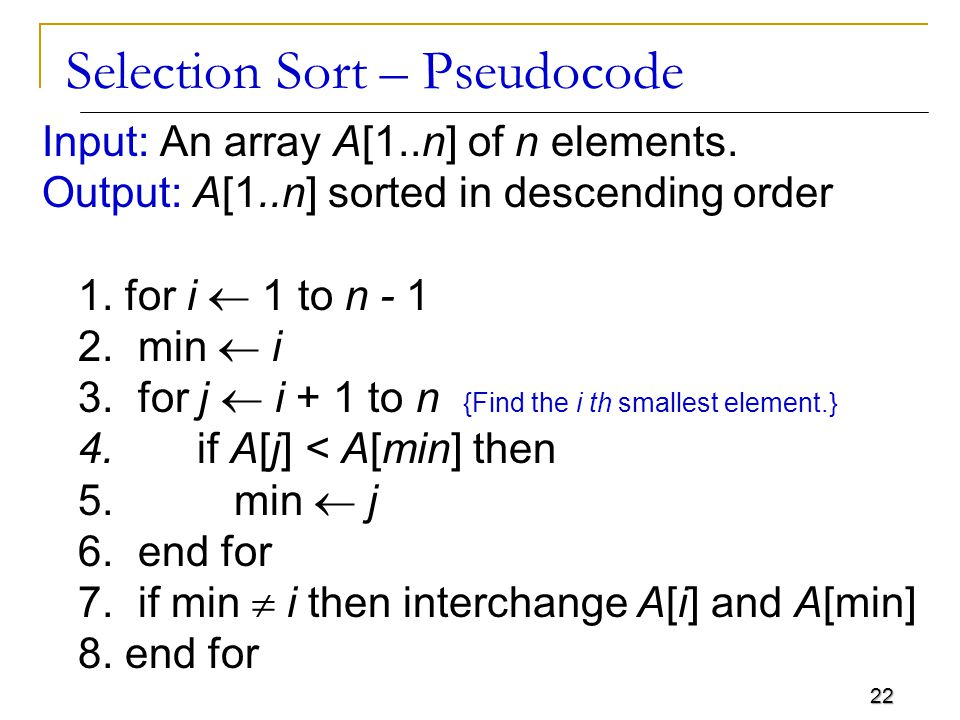
\includegraphics[width=0.5\linewidth]{selection.jpg}
		\caption{The recurrence is $O(n^2)$}
		\label{fig}
\end{figure}
\pagebreak
\item\textbf{Bubble sort: } repeatedly swapping the adjacent elements if they are in wrong order.
\begin{figure}[h]
		\centering
		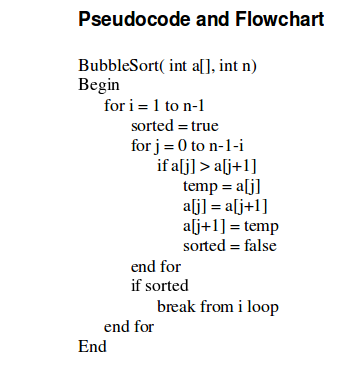
\includegraphics[width=0.4\linewidth]{bubble.png}
		\caption{The recurrence is $O(n^2)$}
		\label{fig}
\end{figure}

\item\textbf{Insertion sort: } Given an array $A[1\ldots n]$ of size $n$, the recursive insertion sort will recursively call on the insertion function for $A[1\ldots n-1]$ until the size of the array is 1, and then insert the last element $A[n]$ into the sorted array of $A[1\ldots n-1]$. The pseudocode for the algorithm is as follows:
\begin{algorithm}[h]
    \SetKwProg{InsertionSort}{InsertionSort}{}{}
    \InsertionSort{($A$, $n$):}{
        \If{$n == 1$}{
            \Return
        }
        \textbf{InsertionSort($A$, $n-1$)}\;
        Set $a = n - 1$\;
        Set $b = a - 1$\;
        Set $temp = A[a]$\;
        \While{$b\leq 1$ and $A[b] > temp$}{
            Set $A[b+1] = A[b]$\;
            Set $b = b-1$\;
        }
        Set $A[b+1] = temp$\;
        \Return
    }
\caption{Insertion sort recursion pseudocode}
\end{algorithm}

The recurrence for the running time of this algorithm is:
\begin{equation*}
  T(n)=\begin{cases}
    1, & \text{if $n = 1$}.\\
    T(n-1) + O (n), & \text{if $n>1$}.
  \end{cases}
\end{equation*}

The time to sort the array if it only contains one element is constant: $T(1) = O(1) = 1$.\\
To sort an array with $n$ elements, we have to sort the array of $n-1$ elements and basically make $n-1$ comparisons as well, bringing us to $T(n) = T(n-1) + (n-1)$.\\
Every iteration until $n=1$, we have to sum up the total operations made at each step, so
\begin{equation*}
    T(n) + T(n-1) + T(n-2) + \ldots + T(1)
    = T(n-1) + T(n-2) + \ldots + T(2) + T(1)
\end{equation*}

\begin{equation*}
    T(n) = T(1) + \dfrac{n(n-1)}{2} = 1 + \dfrac{n(n-1)}{2} = O(n^2)
\end{equation*}

\item\textbf{Heap sort: }Creating a Heap of the unsorted list. Then a sorted array is created by repeatedly removing the largest/smallest element from the heap, and inserting it into the array. The heap is reconstructed after each removal.
\begin{figure}[h]
		\centering
		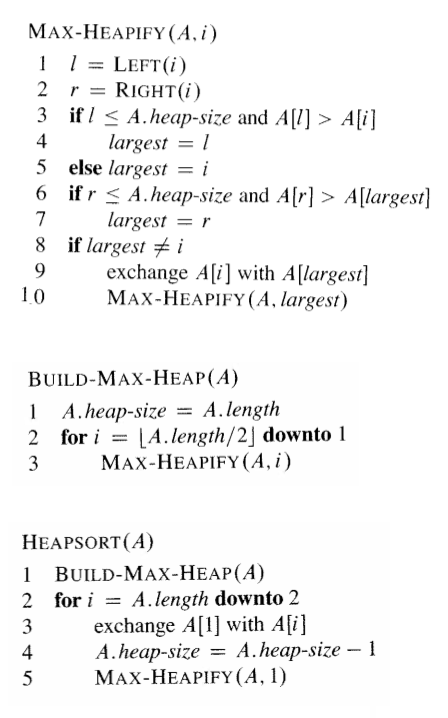
\includegraphics[width=0.4\linewidth]{heap.png}
		\caption{The recurrence is $O(nlog(n))$}
		\label{fig}
\end{figure}

\item\textbf{Quick sort: }The key process in quickSort is partition(). Target of partitions is, given an array and an element x of array as pivot, put x at its correct position in sorted array and put all smaller elements (smaller than x) before x, and put all greater elements (greater than x) after x. All this should be done in linear time.\\
\begin{lstlisting}
/* low  --> Starting index,  high  --> Ending index */
quickSort(arr[], low, high)
{
    if (low < high)
    {
        /* pi is partitioning index, arr[p] is now
           at right place */
        pi = partition(arr, low, high);

        quickSort(arr, low, pi - 1);  // Before pi
        quickSort(arr, pi + 1, high); // After pi
    }
}
\end{lstlisting}

\begin{figure}[h]
		\centering
		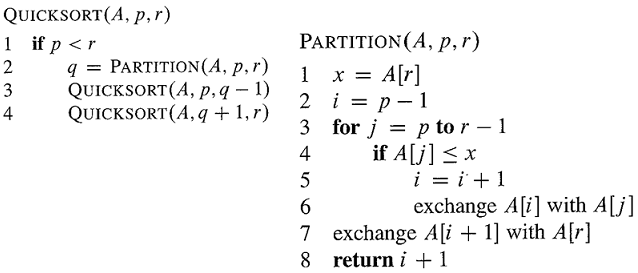
\includegraphics[width=0.7\linewidth]{quick.png}
		\caption{The recurrence is $O(nlog(n))$}
		\label{fig}
\end{figure}
\item\textbf{Merge sort: }Like Merge Sort, QuickSort is a Divide and Conquer algorithm. It picks an element as pivot and partitions the given array around the picked pivot. There are many different versions of quickSort that pick pivot in different ways.\\
The key process in quickSort is partition(). Target of partitions is, given an array and an element x of array as pivot, put x at its correct position in sorted array and put all smaller elements (smaller than x) before x, and put all greater elements (greater than x) after x. All this should be done in linear time.

\begin{figure}[h]
		\centering
		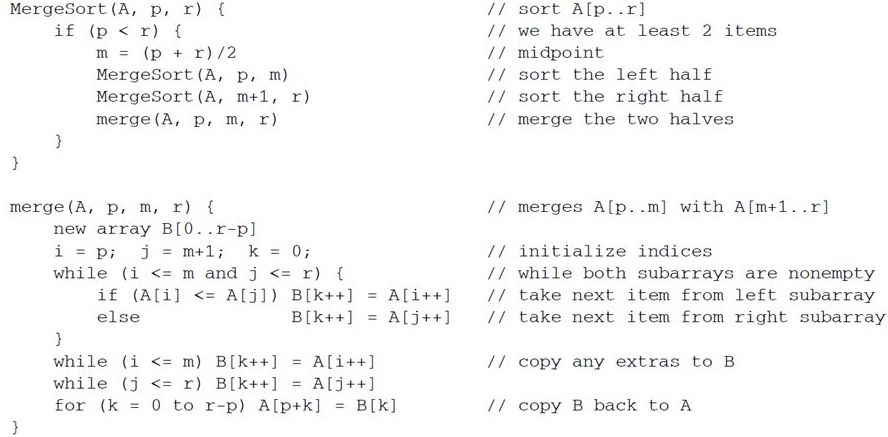
\includegraphics[width=0.7\linewidth]{merge.jpg}
		\caption{The recurrence is $O(nlog(n))$}
		\label{fig}
\end{figure}
\end{itemize}
\end{homeworkProblem}

\end{document}